\documentclass[black,white]{beamer}
\usepackage{beamerthemesplit}
\usepackage{amsmath}
\usepackage{adjustbox}
\usepackage{bookmark}
\usepackage{courier}
\usepackage[T1]{fontenc}
\usepackage{hyperref}
\usepackage[utf8]{inputenc}
\usepackage{listings}
\usepackage{lmodern}
\usepackage{tikz}
\usepackage{hyperref}
\usepackage{listings}
\usepackage{lmodern}
\usepackage{pifont}
\usepackage{subcaption}
\usepackage{svg} % Requires inkscape
\usepackage{tabularx}
\usepackage{tikz}
\usetikzlibrary{mindmap}
\usepackage{verbatim}
\usepackage{xcolor}
\usepackage{yaml}

\beamertemplatenavigationsymbolsempty
\usecolortheme{dove}
\useoutertheme{infolines}
\useinnertheme{rectangles}

\newcommand{\cmark}{\ding{51}}%
\newcommand{\bigcmark}{{\large\textcolor{green}\cmark}}
\newcommand{\xmark}{\ding{55}}
\newcommand{\bigxmark}{{\large\textcolor{red}\xmark}}
\newcommand\blfootnote[1]{%
  \begingroup
  \renewcommand\thefootnote{}\footnote{#1}%
  \addtocounter{footnote}{-1}%
  \endgroup
}

%\makeatletter
%\def\blfootnote{\xdef\@thefnmark{}\@footnotetext}
%\makeatother

\definecolor{ashgrey}{rgb}{0.7, 0.75, 0.71}
\definecolor{charcoal}{rgb}{0.21, 0.27, 0.31}
\definecolor{powderblue}{rgb}{0.69, 0.88, 0.9}
\definecolor{layerblue}{RGB}{213, 234, 254}
\newcommand\sectioncolor{\setbeamercolor{background canvas}{bg=layerblue}}

% Align hash to font
\let\oldhash\#%
\DeclareRobustCommand{\#}{\adjustbox{valign=B,totalheight=.57\baselineskip}{\oldhash}}%

\newcommand{\link}[1]{{\large\color{blue}\href{#1}{#1}}}

% Support backup slides with their own numbering scheme
\newcommand{\backupbegin}{
   \newcounter{finalframe}
   \setcounter{finalframe}{\value{framenumber}}
}
\newcommand{\backupend}{
   \setcounter{framenumber}{\value{finalframe}}
}

\title[Scaling container policy with eBPF]{Scaling container policy management\newline with kernel features}
\institute{Cilium.io}
\author[Joe Stringer]{Joe Stringer}

\setbeamertemplate{footline}
{
    \leavevmode%
    \hbox{%
        \begin{beamercolorbox}[wd=.333333\paperwidth,ht=2.25ex,dp=1ex,center]{author in head/foot}%
            \usebeamerfont{author in head/foot}\insertshortauthor
        \end{beamercolorbox}%
        \begin{beamercolorbox}[wd=.333333\paperwidth,ht=2.25ex,dp=1ex,center]{title in head/foot}%
            \usebeamerfont{title in head/foot}\insertshorttitle
        \end{beamercolorbox}%
        \begin{beamercolorbox}[wd=.333333\paperwidth,ht=2.25ex,dp=1ex,right]{date in head/foot}%
            \usebeamerfont{date in head/foot}\insertshortdate{}\hspace*{2em}
            \insertframenumber{} / \inserttotalframenumber\hspace*{2ex}
        \end{beamercolorbox}}%
        \vskip0pt%
}

\newcommand\newsectionpage[1]{
    \section*{}
    {\sectioncolor
        \begin{frame}
            \vfill
            \centering
            \section{#1}
            \begin{beamercolorbox}[sep=8pt,center,shadow=true,rounded=true]{title}
                \usebeamerfont{title}\insertsectionhead\par%
            \end{beamercolorbox}
            \vfill
        \end{frame}
    }
    \section*{#1}
}

\newcommand\suspense{
    \pause $\rightarrow$
}

\date[Sep 11, 2019]{Linux Plumbers 2019, Lisbon, Portugal}

\begin{filecontents*}{../sw-l3-l4-policy.yaml}
import{../sw-l3-l4-policy.yaml}
\end{filecontents*}

\begin{filecontents*}{../sk-assign.c}
import{../sk-assign.c}
\end{filecontents*}

\begin{document}
    \section*{}
    {\sectioncolor
    \begin{frame}
        \titlepage
        \begin{figure}
            
\includegraphics[scale=0.2]{lpc-logo.png}
        \end{figure}
    \end{frame}
    }

    %\logo{\includesvg[scale=0.4]{cilium-logo.svg}}

    \begin{frame}{Overview}
        \tableofcontents
    \end{frame}

    \section{Background}

    \begin{frame}{Cilium}
        \begin{table}
            \begin{subtable}[l]{0.45\textwidth}
                %\begin{itemize}
                %    \item \textbf<2>{Plumb local connectivity} \medskip
                %    \item Connect remote nodes \medskip
                %    \item Services / loadbalancing \medskip
                %    \item \textbf<2>{Network policy} \medskip
                %\end{itemize}
                %\begin{itemize}
                %    \item Native BPF dataplane \medskip
                %        % BPF -> Awesome, performance, flexibility
                %    \item Modular architecture \medskip
                %        % Modular -> Integrate with your existing tools
                %    \item API-aware authorization \medskip
                %        % L7 security -> More secure
                %    \item Scalability \medskip
                %        % Deploy more and bigger clusters
                %\end{itemize}
                \begin{itemize}
                    \item Native eBPF dataplane \medskip
                    \item Plumb connectivity \medskip
                    \item Identity-based security \medskip
                    \item Scalable \medskip
                \end{itemize}
            \end{subtable}
            \begin{subtable}[r]{0.5\textwidth}
                \begin{figure}
                    \includesvg[width=1.1\textwidth,keepaspectratio]{cilium-plugins.svg}
                \end{figure}
            \end{subtable}
        \end{table}
    \end{frame}

    %\begin{frame}{Kubernetes networking plugins}
    %    \begin{table}
    %        \begin{subtable}[l]{0.6\textwidth}
    %            \begin{itemize}
    %                \item Plumb local connectivity (CNI) \medskip
    %                \item Connect remote nodes \medskip
    %                \item Services / loadbalancing \medskip
    %                \item Network policy \medskip
    %            \end{itemize}
    %        \end{subtable}
    %        \begin{subtable}[r]{0.35\textwidth}
    %            \begin{figure}
    %                \includesvg[width=0.4\textwidth,keepaspectratio]{cni-logo.svg}
    %            \end{figure}
    %        \end{subtable}
    %    \end{table}
    %    \blfootnote{{\tiny \url{https://kubernetes.io/docs/concepts/extend-kubernetes/compute-storage-net/network-plugins/}}}
    %\end{frame}

    \begin{frame}{Kubernetes Architecture 101}
        \centering
        \vfill
        \begin{figure}
            \includesvg[width=0.8\textwidth,keepaspectratio]{k8s-architecture.svg}
        \end{figure}
        \vfill
        \blfootnote{{\tiny Thomas Graf, {\em Scaling to 5k Kubernetes Nodes: Lessons Learned}, Cloud Native Rejekts EU 2019}}
    \end{frame}

    %\begin{frame}{Cluster events}
    %    \begin{itemize}
    %        \item Nodes $\rightarrow$ Fabric connectivity \medskip
    %        \item \textbf<2>{Pods} $\rightarrow$ End-to-end connectivity \medskip
    %        \item Services $\rightarrow$ Logical connectivity \medskip
    %        \item \textbf<2>{Network policies} $\rightarrow$ Connectivity isolation \medskip
    %    \end{itemize}
    %\end{frame}

    \begin{frame}{What does it mean to scale?}
        \begin{itemize}
            \item Minimize unnecessary events \smallskip
            \begin{itemize}
                \item Reduce load on centralized components \medskip
                \item Minimize event sizes \medskip
            \end{itemize}
            \item Apply datapath changes quickly \medskip
            \item Without consuming all available resources \medskip
            %\item Roll out bursty workloads quickly \medskip
            %\item Reduce time from policy change to enforcement \medskip
        \end{itemize}
    \end{frame}

    \newsectionpage{Pod event processing}

    \begin{frame}{BPF plumbing}
        \centering
        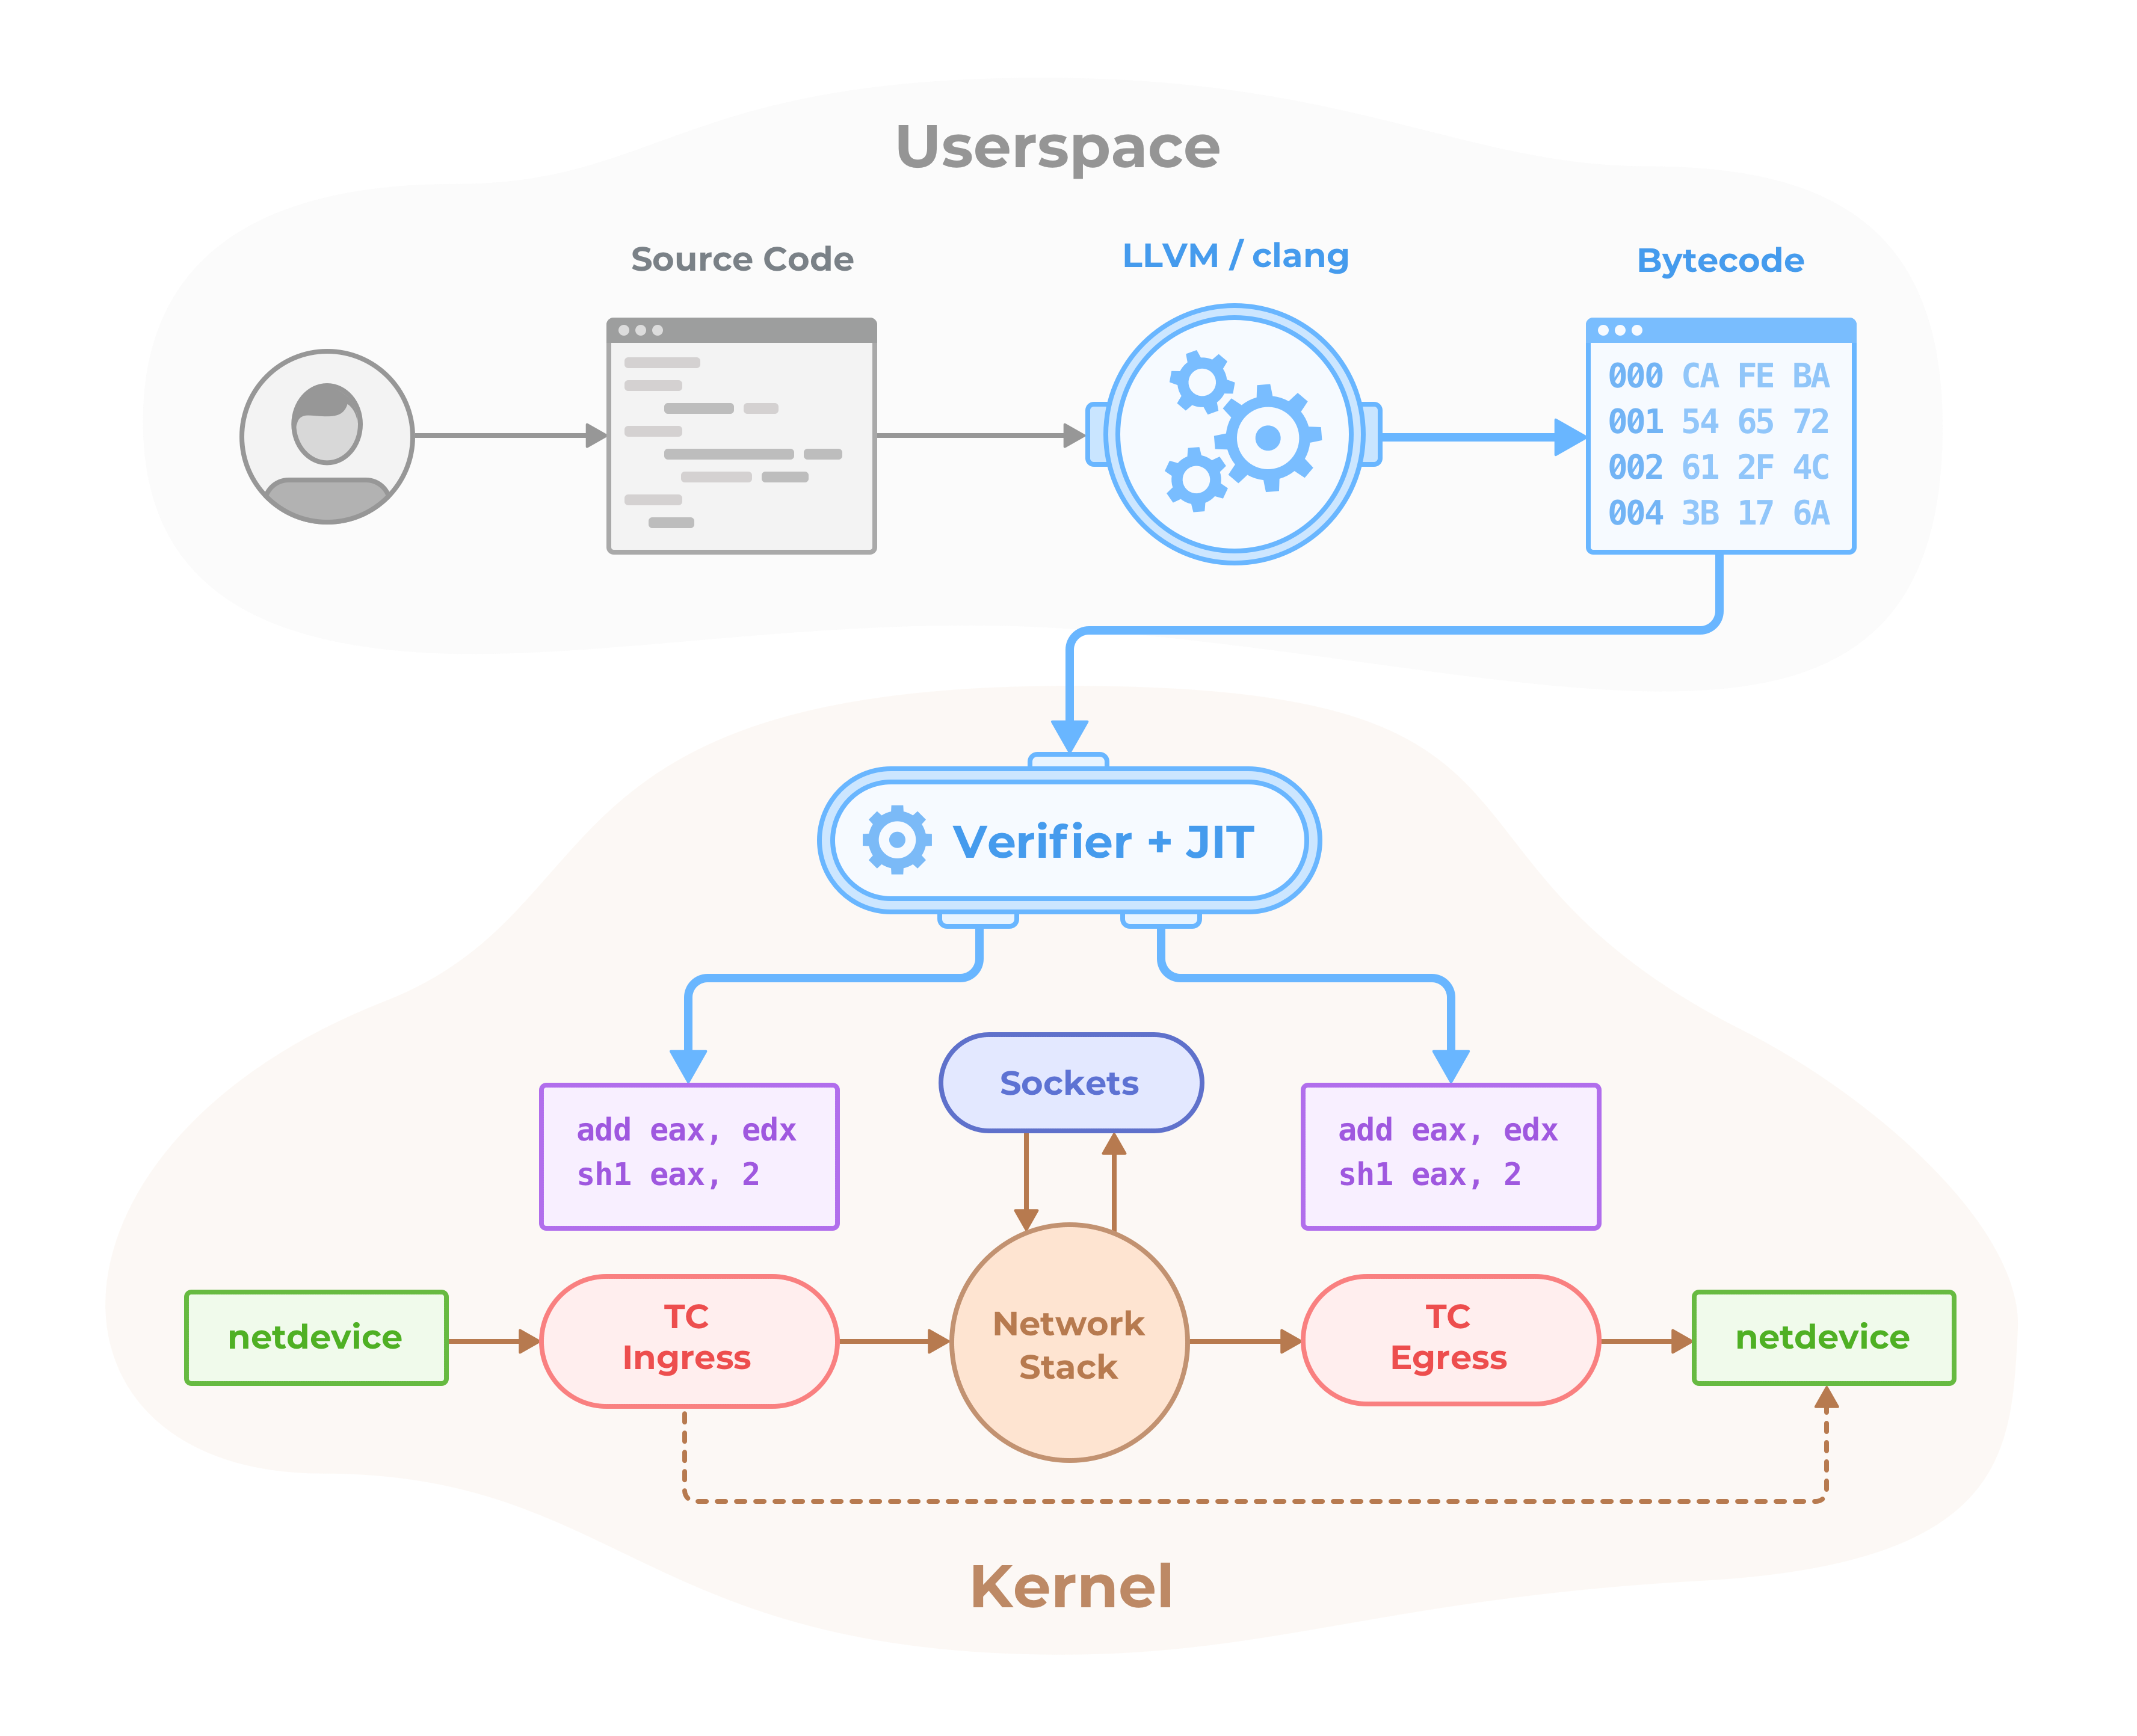
\includegraphics[width=0.8\textwidth,keepaspectratio]{bpf-verifier.png}
    \end{frame}

    %\begin{frame}{Cilium Architecture}
    %    \centering
    %    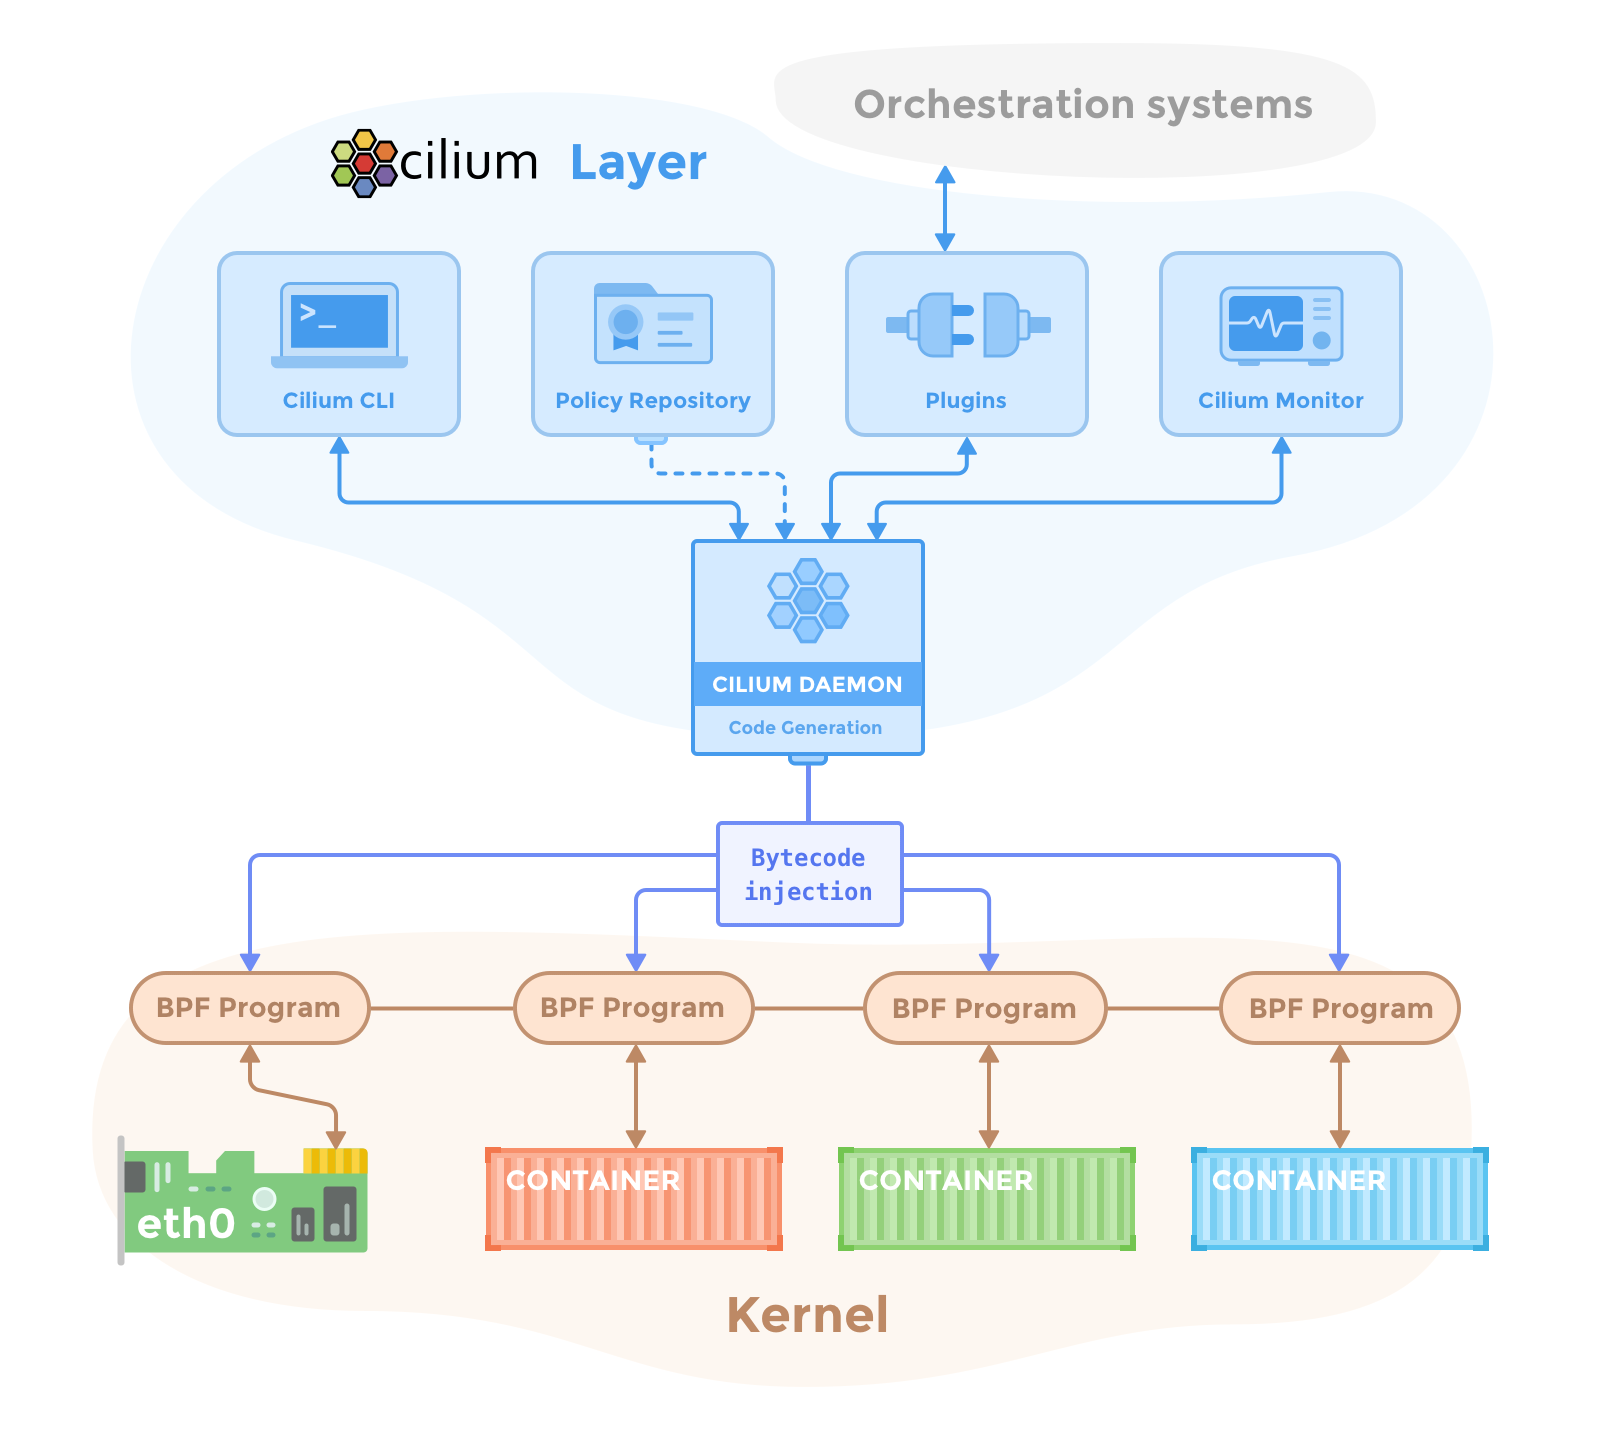
\includegraphics[width=0.8\textwidth,keepaspectratio]{cilium_architecture.png}
    %\end{frame}

    \begin{frame}{ELF Templating}
        \centering
        \includesvg[width=\textwidth]{bpf-templating.svg}
    \end{frame}

    \begin{frame}{1K nodes: Scaling to 60k pods}
        \centering
        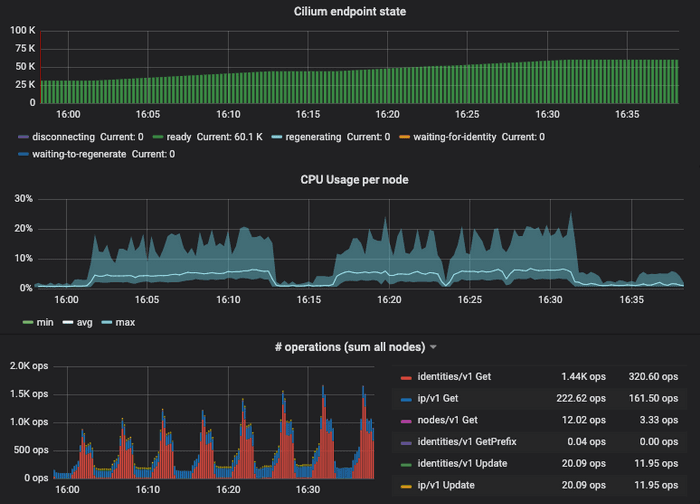
\includegraphics[width=0.8\textwidth]{scaling_to_60k_pods.png}
    \end{frame}

    \newsectionpage{Identity-based security}

    \begin{frame}
        \centering
        \vfill
        % What's going on here?
        \begin{figure}
            \includesvg[width=\textwidth]{identity-security.svg}
        \end{figure}
        \vfill
        \blfootnote{{\tiny Thomas Graf, {\em Cilium \& BPF - The Future of Networking and Security}, openSUSE Conference 2019}}
    \end{frame}

    %\begin{frame}{Policy model}
    %    \begin{itemize}
    %        \item Whitelist \medskip
    %        \pause
    %        \item L3 \smallskip
    %            \begin{itemize}
    %                \item Pod labels \medskip
    %                \item FQDN \medskip
    %                \item Services \medskip
    %            \end{itemize}
    %        \pause
    %        \item L4 \medskip
    %        \pause
    %        \item L7 \smallskip
    %            \begin{itemize}
    %                \item HTTP \medskip
    %                \item DNS \medskip
    %                \item Your protocol here \medskip
    %            \end{itemize}
    %    \end{itemize}
    %\end{frame}

    \begin{frame}{Policy example}
        \lstinputlisting[language=yaml,%
                         showstringspaces=false,%
                         basicstyle=\footnotesize,%
                         breaklines=true]{../sw-l3-l4-policy.yaml}
        \blfootnote{\tiny \url{https://docs.cilium.io/en/stable/gettingstarted/http/}}
    \end{frame}

    \begin{frame}[fragile]{Label selectors}
        \vfill
        \begin{itemize}
            \item 12345 \verb+{org:empire, class:deathstar}+ \smallskip
            \item 12468 \verb+{org:empire, class:tiefighter}+ \smallskip
            \item 12465 \verb+{org:alliance, class:xwing}+ \smallskip
        \end{itemize}
        \vfill
        \begin{tabularx}{\textwidth}{l|l}
            \hline
            & \\
            \verb+matchLabels:+ & 12345 \verb+{org:empire, class:deathstar}+ \\
            \verb+    org: empire+ & 12468 \verb+{org:empire, class:tiefighter}+ \\
            & \\
            \hline
            & \\
            \verb+matchLabels:+ & \\
            \verb+    org: empire+ & 12345 \verb+{org:empire, class:deathstar}+ \\
            \verb+    class: deathstar+ & \\
            & \\
            \hline
        \end{tabularx}
        \vfill
    \end{frame}

    \begin{frame}{Datapath Configuration: Ingress}
        \vfill
        \begin{figure}
            % In the case of ingress policy, by this point it's quite simple.
            % We calculated the necessary allowed identities, just put it in
            % the map.
            %
            % In actuality, this was a simple example but as the number of
            % identities in the cluster rises, and the policy complexity
            % increases, the policy computation can end up becoming quite
            % expensive so we need to be intelligent about how we compute it.
            % Won't go into detail here.
            \includesvg[width=\textwidth]{cilium-bpf-policy-0.svg}
        \end{figure}
        \vfill
    \end{frame}

    \begin{frame}{Datapath Configuration: Egress}
        \vfill
        \begin{figure}
        \begin{overprint}
            % Egress policy is a bit more elaborate.
            % - Ingress case you can transfer the identity with the packet.
            % - Egress you have to choose:
            %   * Defer egress policy apply to the destination
            %     -> Requires destination to know policy of all pods
            %   * Apply egress policy at source, but needs to know identity
            %     of destination
            %     -> Turns out this is much simpler:
            %        + When a pod spins up and gets an identity, push ip-id
            %          mapping to kvstore.
            \onslide<1>\includesvg[width=\textwidth]{cilium-bpf-policy-1.svg}
            \onslide<2>\includesvg[width=\textwidth]{cilium-bpf-policy-2.svg}
        \end{overprint}
        \end{figure}
        \vfill
    \end{frame}

    %\begin{frame}{Policy memoization}
    %    \begin{itemize}
    %        \item Inspired by kernel RCU \medskip
    %        \item Track unique policy selectors \medskip
    %        \item Atomically replace identity selections \medskip
    %        \item Notify policy handlers for BPF update \medskip
    %    \end{itemize}
    %\end{frame}

    %\begin{frame}{Accessing remote resources}
    %    \begin{itemize}
    %        \item Labels are only valid within the cluster \medskip
    %        \item DNS is a kind of label... \medskip
    %        \item Proxy DNS, associate IPs to FQDNs \medskip
    %        \item Bonus: Identity mapping can be local \medskip
    %    \end{itemize}
    %\end{frame}

    %\begin{frame}[fragile]{FQDN selectors}
    %    \vfill
    %    \begin{itemize}
    %        \item 168402 \verb+{cidr:192.0.2.3}+ \smallskip
    %        \item 168624 \verb+{cidr:192.0.2.4}+ \smallskip
    %    \end{itemize}
    %    \vfill
    %    \begin{tabularx}{\textwidth}{ l|l}
    %        \hline
    %        & \\
    %        \verb+toFQDNs:+ & 168402 \verb+{cidr:192.0.2.3}+ \\
    %        \verb+     cantina.empi.re + & 168624 \verb+{cidr:192.0.2.4}+ \\
    %        & \\
    %        \hline
    %    \end{tabularx}
    %    \vfill
    %\end{frame}

    \newsectionpage{Layer 7 security}

    \begin{frame}{L7 is the new L4}
        \vfill
        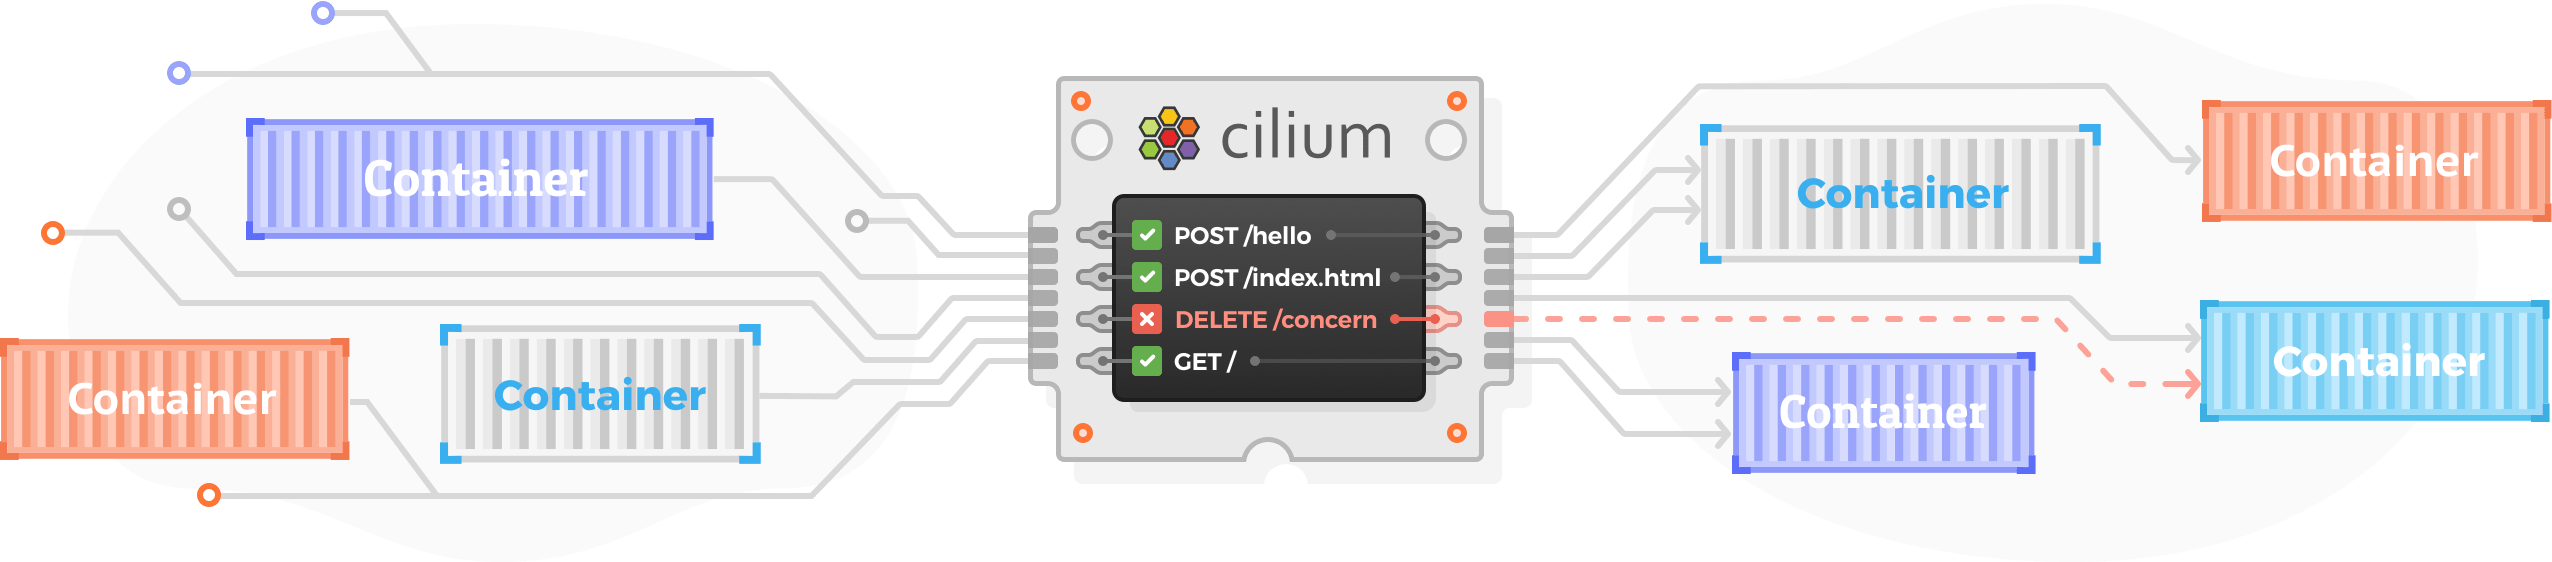
\includegraphics[width=\textwidth]{cilium_api_security.png}
        \vfill
    \end{frame}

    \begin{frame}{Datapath Configuration: L3 flow}
        \vfill
        \begin{figure}
            \onslide<1>\includesvg[width=\textwidth]{cilium-bpf-egress-l3.svg}
        \end{figure}
        \vfill
    \end{frame}

    \begin{frame}{Datapath Configuration: L7 flow}
        \vfill
        \begin{figure}
        \begin{overprint}
            \onslide<1>\includesvg[width=\textwidth]{cilium-bpf-egress-l7.svg}
            \onslide<2>\includesvg[width=\textwidth]{cilium-bpf-egress-proxy.svg}
        \end{overprint}
        \end{figure}
        \vfill
    \end{frame}

    \begin{frame}{L7 Configuration: Past}
        \centering
        % TODO: Clean up this
        \onslide<1>{\footnotesize Per-endpoint configuration}
        \onslide<1->
        \begin{overprint}
            % First: Lots of configuration.
            % - Various control messaging with proxy.
            % - Synchronization between agent and proxy for policy map plumbing
            % - Proxy configuration failure handling
            \onslide<1>\includesvg[width=\textwidth]{bpf-proxy-nat-0.svg}
            \onslide<2>\includesvg[width=\textwidth]{bpf-proxy-nat-1.svg}
            % Rewrite destination, update checksums, etc.
            % - Great, now it's directed towards the local proxy instance
            \onslide<3>\includesvg[width=\textwidth]{bpf-proxy-nat-2.svg}
            % Uh-oh, we lost our actual destination.
            % - Let me just fix that up...
            % - New bpf map, proxymap!
            % - Make proxy aware of this map to read the original destination
            \onslide<4>\includesvg[width=\textwidth]{bpf-proxy-nat-3.svg}
            % OK, so where are we at?
            % - It works (yay)
            % - Configuration is costly, per-port
            % - Per-packet NAT seems a bit unnecessary, we know it's destined
            %   locally
            % - Maintaining this extra proxymap for transferring metadata
            %   between kernel and userspace seems a bit icky
            \onslide<5>\includesvg[width=\textwidth]{bpf-proxy-nat-4.svg}
        \end{overprint}
        % TODO: Clean up this
        A: 192.0.2.3:33333 ; B: 192.0.2.4:80 ; L: 192.0.2.1:12345
    \end{frame}

    \begin{frame}{L7 Configuration: Present}
        \centering
        \begin{overprint}
            % What's the alternative? Transparent sockets!
            % - Requires a bit of proxy work, but hey we only need one listener
            % - Every port for the same protocol can go over the same proxyport
            \onslide<1>\includesvg[width=\textwidth]{bpf-proxy-tproxy-0.svg}
            % Theme: Shakespeare
            %
            % Gonna require a bit more kernel configuration...
            % - A sprinkling of netfilter
            % - A dash of policy routing
            % - Watch out for the mark of the beast...
            \onslide<2>\includesvg[width=\textwidth]{bpf-proxy-tproxy-1.svg}
            % ...and there it is.
            % - In BPF, we mark the packet for tproxying
            % - In PREROUTING we match on the mark and look up the proxy port
            % - Actually going to need another mark..
            \onslide<3>\includesvg[width=\textwidth]{bpf-proxy-tproxy-2.svg}
            % Set up policy routing
            % - IP rule to match the mark, choose a route table..
            % - And configure that route table to always route locally
            \onslide<4>\includesvg[width=\textwidth]{bpf-proxy-tproxy-3.svg}
            % Home free!
            \onslide<5>\includesvg[width=\textwidth]{bpf-proxy-tproxy-4.svg}
        \end{overprint}
    \end{frame}

    \begin{frame}{L7 Configuration: Proposal}
        \centering
        \begin{overprint}
            % How about... we put this in BPF
            % - Discussed at LSFMM, which lead to two directions
            % - Monday discussion slot by CF
            % - Socket assign, as follows...
            \onslide<1>\includesvg[width=\textwidth]{bpf-proxy-demux-1.svg}
            % Started looking at this, it looks like sk_assign
            % - Socket lookup was introduced in v4.20
            % - New: sk_assign
            % - Oh and we need our magic marks
            \onslide<2>\includesvg[width=\textwidth]{bpf-proxy-demux-2.svg}
        \end{overprint}
    \end{frame}

    \begin{frame}[fragile]{Socket assign: RFC}
        \centering
        \lstinputlisting[language=c,%
                         showstringspaces=false,%
                         basicstyle=\scriptsize,%
                         breaklines=true]{../sk-assign.c}
    \end{frame}

    \begin{frame}[fragile]{Socket assign: Hiccup}
        \centering
        \begin{itemize}
            \item BPF progs are attached at TC ingress \medskip
            \item \verb+skb_orphan()+ invoked directly before \verb+PREROUTING+ \medskip
            \pause
            \item TC folks are already carrying hacks for this\footnotemark \medskip
            \pause
            \item Just move to \verb+____dev_forward_skb()+\footnotemark? \medskip
        \end{itemize}
        \footnotetext[1]{\tiny \url{https://www.mail-archive.com/netdev@vger.kernel.org/msg303851.html}}
        \footnotetext[2]{\tiny \url{https://www.mail-archive.com/netdev@vger.kernel.org/msg304057.html}}
    \end{frame}

    \begin{frame}{L7 Configuration: Socket redirect}
        \includesvg[width=\textwidth]{bpf-proxy-demux-3.svg}
    \end{frame}

    \begin{frame}{Summary}
        \begin{itemize}
            \item Minimize processing cost \smallskip
            \begin{itemize}
                \item Number of events \medskip
                \item Cost for each event \medskip
            \end{itemize}
            \item Separate concerns: Policy vs addressing \medskip
            \item Frontload expensive operations \medskip
            \item ... while keeping runtime costs low \medskip
        \end{itemize}
    \end{frame}

    \section*{}
    \begin{frame}{Thank you}
        \centering
        \vfill
        \begin{table}
            \begin{subtable}[l]{0.6\textwidth}
                \begin{tabular}{rl}
                    \multicolumn{2}{l}{\textbf{More information}} \\ \\
                    \includesvg[width=0.045\textwidth]{www.svg}
                    & \link{https://cilium.io} \\
                    \includesvg[width=0.045\textwidth]{slack.svg}
                    & \link{https://cilium.io/slack} \\
                    \includesvg[width=0.045\textwidth]{github.svg}
                    & \link{https://github.com/cilium/cilium} \\
                    \includesvg[width=0.045\textwidth]{twitter.svg}
                    & \link{https://twitter.com/ciliumproject} \\
                \end{tabular}
            \end{subtable}
            \begin{subtable}[r]{0.35\textwidth}
                \includesvg[width=0.9\textwidth]{cilium-gopher.svg}
            \end{subtable}
        \end{table}
        \pause
        \vfill
    \end{frame}

    \appendix
    \backupbegin
    \begin{frame}{Socket redirect}
        \includesvg[width=\textwidth]{bpf-proxy-demux-3.svg}
    \end{frame}

    \begin{frame}[fragile]{Socket assign: API quirks}
        \centering
        \begin{itemize}
            \item Nit: Need to use \verb+sock_common+ socket lookups \medskip
            \item Add \verb+bpf_skc_lookup_udp()+ \medskip
            \item Optimization: Add lookup flags to \verb+bpf_sk*_lookup_*()+ \medskip
        \end{itemize}
    \end{frame}
    \backupend

\end{document}
